\subsection{CRUD}

\todo{insert node02 graph}
The main focus of this sprint was to get the server up and running for the other layers. 
As we already had a working database, the goal of this increment became to write a CRUD api through HTTP, 
the other layers could use to acces the database.
The CRUD operations we implemented are based on requests from the other layers, and what they thought they needed to retrieve from the database.

To implement this we split the CRUD operations into three different API's handling different aspects of the database.

\begin{figure} \centering
   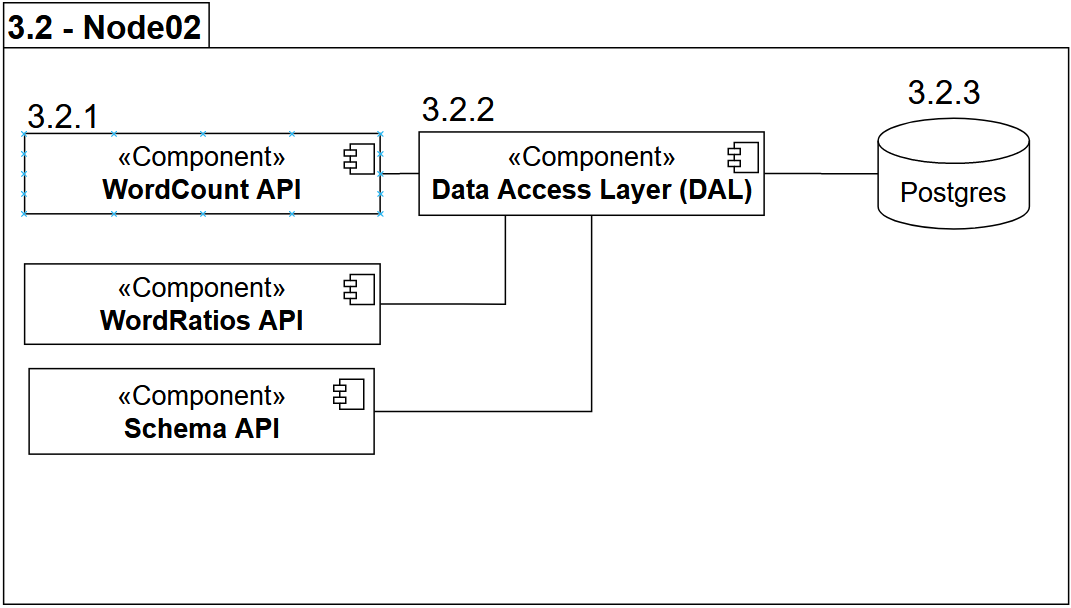
\includegraphics{Images/Node02Sprint3.PNG}
   \caption{Node2 sprint 3}
   \label{Node02Sprint3}
\end{figure}

\subsubsection{WordCount API}
The first API was the wordcount API, which has implemented two Get methods.
The first method called GetAll() retrieves all the words currently stored in the database.
Another method called Get() takes a word as an argument and checks wether that word already exist in the database.
In the WordCount API we also implemented a Post method called Post() which takes a json object from the HTTP body as a parameter. 
The Json object should correspond to an array of articles which will then be posted to the database. 
The method checks wether key information or words already exists in the database, 
and the input mathces JSONschema from the database before adding the item.


\subsubsection{Wordratios API}
The second API is the WordRatios API. which only has one get method.
The method gets all entries in the WordRatios table. 

\subsubsection{Schema API}

The last API we implemented in this iteration is the Schema API which is used to post a JSON schema to the database, which is later used to verify JSON objects.
The route to this endpoint is simply \texttt{/Schema}. 
The body of the post request must consist of two fields - the schema name, which is its primary key in the database, and the schema content itself. 
A schema gets stored in the database in the format known as \texttt{jsonb} or JSON binary which is a built-in type provided by \postgres{}.
This format is used to store a JSON object as binary which uses much less space than a varchar or regular JSON type would.

% Create, Read, Update, Delete
% vi har implementeret CRUD operationer til databasen som de andre lag kan bruge.
    % get
        %All wordRatios
            % why?
        % get all words
            % why?
        % get word by word
            % checks if a word exists
            % why do we have it
    % post
        % post articles as json
            % checks if the input matches a jsonschema from the DB
            % checks if an article name exists
            % checks if a filepath exists
            % checks if a word exists 
        % post Jsonschema
    % Jsonschema

\todo{Mention earlier that the database was accesed directly, instead of through an API}
\todo{describe the structure of the database}


We chose not to implement the update and delete function to our API's in this increment, 
because it was not strictly needed to make the search engine work.



%Deliverable, implementation and documentation
%During this increment we will.... description of results of the implementation and needed documentation / theory. 
%Backlog overview / fulfilment
%updated diagrams


% Entity framework
    % Hvad er Object relational mapping (ORM) tool
    % EF vs dapper?
    % hvad er EF
    % hvorfor bruger vi det
    
% postgresql
    % hvad er det
    % hvorfor bruger vi det
        % det vi lærer i kurserne
        % det er hvad der var på databasen i forvejen



% --Implementation--
% Docker
    % hvad bruger vi det til
        % Test DB
    % hvordan har vi implementeret det

% Entity framework
    % hvad bruger vi det til
        % lige nu til at tilgå elementer i databasen
        % svært at bruge med den nuværende struktur på databasen
        % i fremtiden vil vi også generere en ny database med EF for at have en code first approach

% postgresql
    % Vi har unmaterialised et view

% vores fokus har været på at få serveren op at køre med de andre lag, 
% derfor har vi hovedsagligt arbejdet på at få nogle APIer op at køre